\documentclass[10pt]{article}
\setlength{\topmargin}{-0.8in}
\setlength{\textheight}{9.5in}
\setlength{\oddsidemargin}{-.13in}
\setlength{\textwidth}{6.5in}

\usepackage{multirow}
\usepackage{array}
\newcolumntype{L}{>{\centering\arraybackslash}m{3cm}}

\usepackage{graphicx}
\graphicspath{{images/}}

\begin{document}

\title{A User Model for People with Autism within Search }
\author{Esha Massand\\
MSc Computer Science Project Proposal\footnote{This proposal is substantially the result of my own work, expressed in my own words, except where explicitly indicated in the text. I give my permission for it to be submitted to the JISC Plagiarism Detection Service. }}
\date{\today}
\maketitle

\begin{abstract}
The current proposal presents my objective to research and build a user model within Search, to address the downfalls of current Search tools for individuals on the Autism Spectrum. The user model will be built around the core features of Autism. The model will be applied to results returned from a synthesis of three leading existing search engines. The final product will be a web application, integrated with motion-controlled user interfaces (UI). These findings will provide novel insights into the needs and wants of individuals with Autism within search, and enable future development and interventions within these information streams and communication channels.
\end{abstract}

\tableofcontents

\section{Introduction \& Background}
\subsection{Problem Statement} \label{prob}
Most search engines apply user models to refine search queries. No research to date has attempted to define a user model within search for individuals with Autism. It is currently unknown whether current user models need to be adjusted for this subgroup of the population. We argue that the user models that underlie the way in which search queries are handled, and the needs of the user differ to the mainstream models. This project aims to build a user model of Autism to address this issue.
As it has been shown that individuals with Autism are more engaged (demonstrate sustained attention) when using technology that is receptive and interactive (e.g., games, responsive consoles, motion controlled devices) compared to technology that is not. This project will combine interactive, motion recognition hardware with Search to improve the UI and architecture of Search for individuals with Autism.

\subsection{The Role of Context In Search}
It is unlikely that any given page on the web will contain a word or phrase that means exactly (or nearly) the same as another word or phrase in that language (e.g., shut and close). How is it then that your search engine of choice picks these phrases to mean the same thing, and returns them synonymously in the results of your query? Well, quite simply put, it is by virtue of the fact that each of their neighbouring words and associations are similar. These are indirect, higher-order associations, and provide the context in which the search engine can index keywords. This context plays a crucial role in search; first, in the interpretation of the user query, and second, it is reflected in the results returned to the user.

\subsection{What is the Autism Spectrum?}
Autism is amongst the most common neurodevelopmental condition and it is currently estimated that 1/68 children meet criteria for Autism Spectrum (CDC, 2014). Autism is five times more common amongst boys than girls (1/42 boys, and 1/189 girls). According to the DSM-V (2013) diagnostic manual, Autism is characterized by persistent and early deficits in reciprocal social interaction and repetitive behaviours. Individuals vary from high functioning to low functioning (along a spectrum), with behaviours emerging around 2 to 3 years of age. 

\begin{center}
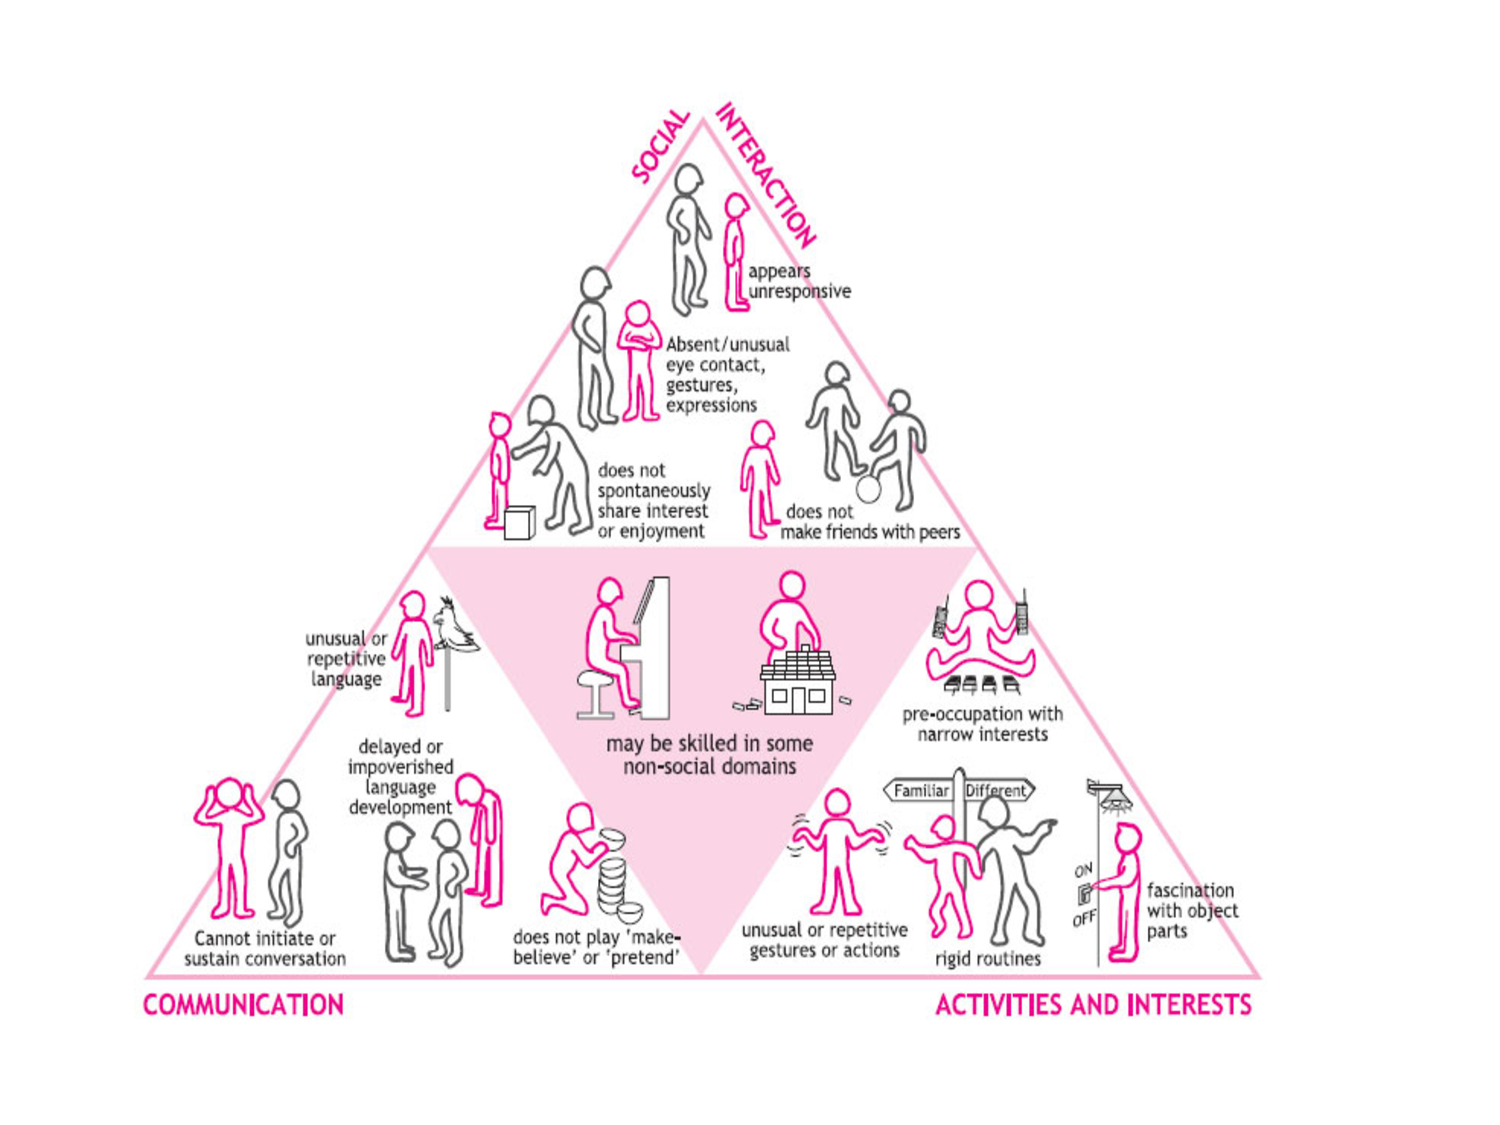
\includegraphics[scale=0.5]{asd}\\
The Autism Triad \cite{triad}
\end{center}


\subsection{Proposal Organisation}

This proposal outlines my research to date on Search, Autism, and Motion Controller interfaces. I also include my preliminary planning of the methods I will use to implement the enhanced Search tool for Autism. The remaining chapters discuss:
\begin{enumerate}
\item in Section~\ref{What should Search offer people with Autism}, I give a brief introduction to Search engines, and the downfalls of current Search engines for individuals with Autism. I discuss the motivation behind the proposed work
\item in Section~\ref{usermodel}, I discuss the potential for user modeling within Search
\item in Section~\ref{Existing Combination/Advanced Search Engines} I review current existing combination search engines 
\item in Section~\ref{proposed} I outline my proposed search application
\item in Section~\ref{api}, I briefly discuss the API's and Libraries that I will use during the project, including my research on Custom Search Engine APIs such as the Google Custom Search API, and Yahoo BOSS, Bing Search API, Apache Lucene Key Word In Context
\item in Section~\ref{hardware} I review the LEAP motion controller hardware and SDK that I aim to integrate with the search application
\item in Section~\ref{plan} I outline my project plan, and
\item in Section~\ref{future} I discuss the future directions and implications of this research.
\end{enumerate}



\subsection{What should Search offer people with Autism?}\label{What should Search offer people with Autism}
\subsubsection{Search and Learning}
The Internet is one of the largest resources of information, and can be searched by users from different areas of the world relatively quickly. Search engines allow users to collate hundreds of links on a single topic, using only a few words or phrases. The information returned is vast, and requires the user to sort the returned results into 'relevant' or 'irrelevant' categories. This requires the user to flexibly shift between one result and the next, to determine the relevance of each page returned by the search engine. Search allows the user to extrapolate the information on the page into their knowledge and is an important learning tool; its significance is duly noted because of the learning benefits it brings for children and adolescents as they begin to navigate the Internet and gain an understanding of several subjects. 

\subsubsection{Clues from virtual reality and gaming}
Almost all teenagers (97\% of those aged 12-17) use a computer, web, portable or console device, 73\% of which is desktop/laptop based. Teenagers with Autism also use technology and spend a substantial amount of their time using devices \cite{Shane and Albert}. They are proficient and use these devices with relative ease, showing high levels of engagement with consoles like the Xbox (Kinect) or Wii, Portable Gaming Devices (Nintendo DS), or cell phone or handheld devices. For individuals with Autism, computer-based technologies can provide a stable, consistent learning environment that can be customized \cite{moore}. With this in mind, the proposed application will integrate motion controllers into it's design, to facilitate user attention and engagement with Search. 

\subsubsection{Motion Controllers}
Motion recognition devices can be programmed to make consistent responses to environmental triggers. This is unlike real-world situations where environmental responses are not always consistent and may require further interpretation or ‘guess-work’. These controlled and interactive environments have shown promise for improving social communication skills and reducing repetitive behaviours \cite{gameshealth}.

\subsubsection{Visual not text-based}
People with Autism demonstrate stronger visual memory \cite{fabienne} than verbal memory, so a more visually-oriented approach to search (one that doesn’t require sustaining a verbal search query in working memory) is a more appropriate way to present data to bolster the strength of visual memory in people with Autism.

\subsection{Existing Combination/Advanced Search Engines}\label{Existing Combination/Advanced Search Engines}
The first part of the proposed project involves the synthesis of results from three leading search engines. There are several search engines which return combined results to users wishing to conduct a more 'complete' search, four of which are described below. 

\subsubsection{Bing vs Google}
Bing vs. Google presents the users’ search query results from both search engines to allow the user to make a comparison (the Google and Bing results can be presented vertically or horizontally beside each other), and provides the experience of navigating both search pages simultaneously.  
The number of other personal preferences options is very limited (the orientation of the results is just about all the user has the option to choose). There is also double the information on the page (overload), so not a solution for the current project.

\subsubsection{Qrobe.it}
Qrobe combines three search engines’ results (Google, Bing and Ask) and presents them conveniently on one page. Unlike Bing vs Google the user can search ‘web’, ‘images’ or ‘popular’ (to reveal stories from Reddit). Qrobe.it also has a ‘cheat sheet’ that allows user to search using shortcuts, which may prove useful to a seasoned Qrobe user. Qrobe has not got an open (or well tested) API for developers to use to extend its functionality further, meaning it is a riskier option to choose for this project.

\subsubsection{AskBoth}
AskBoth – is a work in progress, and combines both Google and Bing, with a section in the middle dedicated to twitter. AskBoth argues that the selling points for the site are it’s ‘uncomplicatedness’, aesthetics and user experience (UX) – which promises to be particularly good (promised, since 2009).

\subsubsection{Spectra}
Spectra takes searching from Google, Bing and Yahoo engines one-small-step-further. This site allows users to assign weights and determine the way results are displayed. Spectra gathers the search results, ranks them and displays them according to their algorithm. Spectra does not provide an API for developers, and the rigor of the search is hard to test, (not much user data available to analyse).

\subsubsection{Conclusions and ways forward}
These search engines allow users to see more results than what one search engine alone would present. In the circumstance of Bing vs Google, and AskBoth, there is a cost -- redundancy (near-duplicates) and ‘cognitive overload’. This is not ideal for users with Autism, as this is precisely the opposite of what the application's aims and objectives were (see Section~\ref{prob}). In the circumstance of Spectra and Qrobe, there is no Open API available. I will therefore work on the creation and synthesis of the results using the GSC, Bing and Yahoo API's.
The following section proposes an application that will try and address the aims of the current project.

\section{The Problem}\label{the problem}
Search-engine algorithms assume that the user is context-driven, and attempt to model the user's intent using higher-order contextual information gathered from available web pages. This process also models the brain's ability to extract context and semantic associations from information. However, people with Autism are less context-sensitive, preferring a more detail-focused processing style \cite{mottron}. They would intuitively form search queries very differently. Individuals with Autism are also less likely to engage in a relational (hierarchically organized) style of processing \cite{bowler} suggesting that relating information in a hierarchically organised framework is less likely. Hierarchical organisation implies a great deal of flexibility and mental-shifting, as a simple example, in a search for 'apple', it would imply awareness that the word is related to 'pear' but also to 'fruit'. Awareness of this latter relation also suggests awareness that 'apple' is related to 'pomegranate'. This is of course, a simple example, but these associations can get very complex very quickly. Generally speaking, individuals with Autism prefer, and are more likely to engage in an item-specific processing style, and, whilst intelligent cognition is definitely possible, search queries are more likely formed of first-order associations\footnote{Of course there is a great deal of individual variability in the Autism Spectrum.}. \\

\subsection{Aims and Objectives}
Several Psychology learning and intervention studies for individuals with high functioning Autism have suggested that assimilation and accommodation of new information is most appropriate when:\\
\begin{enumerate}
\item Information is concrete (not abstract).
\item Information is presented in contextually-relevant chunks.
\item Information is not verbally "overloaded" (not too many words).
\item Information is presented in a set visual format.
\end{enumerate}
Several interventions have been built around this body of literature (see www.autismspeaks.org).
Given these findings from the literature we can make several adjustments to current Search tools to enhance their benefit for people with Autism. For example:
\begin{enumerate}
\item Assessing the results for the Key Word In (a suitable) Context.
\item Using a similar order of semantic association, in line with the search query itself (precedence for first-order relations). 
\item Smaller snippets and presenting in a more manageable way (less overloaded with words).
\item Visual consistency.
\item A high degree of verbal consistency/similarity with the search query.
\end{enumerate}

This project will \textbf{integrate} these insights from the Psychology literature with the proposed application.


\section{Plan for Developing the Solution}

\subsection {Creating a User Model of Autism}\label{usermodel}
\subsubsection{What is a user model?}
A user model is a collection of information associated with a particular user, with which a system can adapt its behaviour in order to customise in line with the user’s needs. The concept of user modeling has strong implications for the way in which humans and computers interact; by creating a representation of the user, the system can be better informed about how to behave in various circumstances, for example, the system can acknowledge a specific kind of user’s demographics, needs, preferences, likes, dislikes, goals, plans, knowledge, and skill. The system can maintain this knowledge whilst interacting and adapting its behaviour with the user.
Persona development (research-based, user types), will support the user modeling process by identifying particular characteristics of individuals with Autism in Search. An individual’s personal information, will be stored in a user profile which will contain demographic information such as age, gender, lifestyle, frequent tasks, tools used, resources commonly used. The profile will also include information about diagnosis (Autism, Asperger, and high/low functioning).

\subsubsection{Types of user models}
User models can be static, and unchanging (i.e., no algorithms are used in order to teach the model about the changing preferences of the user, and no new information is fed into the model), or dynamic (representation of the user with their up-to-date changes in interests, and recent interactions with the system). Alternatively, user models can be stereotyped. This means they utilise demographic information to classify users into distinct subtypes. The system infers or assumes other characteristics about this subset of users by making use of data gathered from other users also included within this subset. Lastly a user model can be highly adaptive and try to model the one user on their own, without stereotyping or inferring the characteristics of the user. This type of user modeling requires a large amount of data collection prior to its implementation.\\
The model can gather information through direct interaction with its user (e.g., via a registration process), by observing and interpreting the users actions, or, by a combination of both, that is, the system may ask for feedback, and alter its approach depending on the user’s behaviour.\\
I will develop a stereotyped user model in the first instance, with the aim to add functionality and increase the model's adaptivity as it acquires more data via user-interaction.

\subsubsection{Benefits and difficulties of user modeling in Search}
A user model needs to collect data before it can predict the user’s needs with accuracy, but once this is achieved, information can be presented according to the user’s knowledge, ability and goals. It can also effectively filter out irrelevant information and rank the remaining search results in the most relevant way according for the user.
Creating a user model is not an easy task. The designer of the system has to set weights of parameters for the information that is fed into the model, and decide what course of action to take when two pieces of information may conflict. The user model will focus on refining search results based on the presence of first-order, or, item-specific relations to a search query (rather than hierarchical relations). The model will be developed around well-understood cognitive processes in Autism. Other elements of the user model will be decided with user-feedback (during testing). 

\subsubsection{Adaptive / Personalised Search}
Adaptive or Personalised search, is one way in which search engines including Google, Yahoo and Bing have attempted to tailor the search results for their users. The feature was first introduced as part of a GoogleLabs project in 2004 and implemented in 2005. It associates each user search with a HTTP cookie – this is a piece of data (a text file) sent from the website and saved in the users’ browser when the user navigates that website. These cookies contain information such as login information (gender, age), preferences (languages, interests) and other information about previous searches based on site traffic. The cookies allow the website to ‘remember’ stateful information about what buttons the user clicked on, or what sites they visited. This cookie record allows the search engine to return results that are highly relevant to the search query, but also highly relevant to the pages that the user visited through previous searches. When personalised or adaptive search is combined with GPS data from a smartphone or device, it can provide useful information about the places that user has previously visited to higher rank local items in the users returned results. This creates a personalized or adaptive web search, as the feature allows the web search to be tailored to the user’s preferences over the course of time, and as more searches are recorded.

\subsubsection{Disadvantages of Current Adaptive Search for Individuals with Autism}
Although adaptive search seems to have significant user benefit in terms of relevance to the user for that search query, it decreases the likelihood that the user encounters new information and biases the results towards the users location and their previous site traffic.  This has the unwanted effect of creating a filter bubble (Pariser, 2011), which is argued to close us off from important and relevant information and create a personal ecosystem of information for one particular user, creating the impression that “our narrow self interest is all that exists”. The filter bubble also has potential privacy problems, as the user may be unaware that the search has been specifically tailored towards their interests and they wonder why things that they have previously searched for have become more and more relevant. There are search engines that have attempted to address this unwanted effect, by not tracking or saving user information (e.g., DuckDuckGo.com). As users are not linked to their search queries, it limits them being targeted by adverts related to their previous searches. The filter bubble may positively reinforce restricted interests in Autism as the user constantly receives feedback about their previous (idiosyncratic and personalized) searches without being able to break out of that repetitive loop. \\Recent research has suggested personalization also increases ‘background noise’ relative to the search results \cite{briggs}. Briggs (2014) suggests that there is a carry-over effect in personalized search for the users, whereby prior search results influence the results of subsequent searches \footnote{It should be noted that personalization of search results generally takes a lower priority for the ranking algorithms than the URLs ranked top in terms of their relevance for the search query.}.  Nevertheless this carry-over may be particularly disadvantageous for people with Autism (some of whom already have restricted and repetitive interests) as it muddies their search space.\\
In order to produce a search tool specifically tailored to reduce the filter bubble effect in Autism, widen the information gateway and reduce the possibility for restricted and repetitive searches, the weighting on previous search results needs to be reduced. This is something I will investigate in the project, particularly for individuals with restricted interests. For these users, it would limit the possibility that they get trapped in a spiraling loop of ever-narrowing user-relevant information and over personalization of self-reinforced information ecosystems.

\subsubsection{Persisting the User's Information}
The user will be asked to sign in with a Google+ account (providing their demographic information), and the Google+ API will be used to store/retrieve this information about the current user. The API contains methods to access 4 resource  types; People, their Activities, Comments and Moments. A person is represented with many fields in Google +, including name, gender, title, occupation, all of which can be used to model individual users in the current project. Information about web searching history for any individual user can be obtained from the browser history. 



\subsection{Proposed Search and Controller Web Application}\label{proposed}
This project will produce a Search web application designed to enhance the UI and UX within search for people with Autism. Below I list the core and non-core features included:

\begin{center}
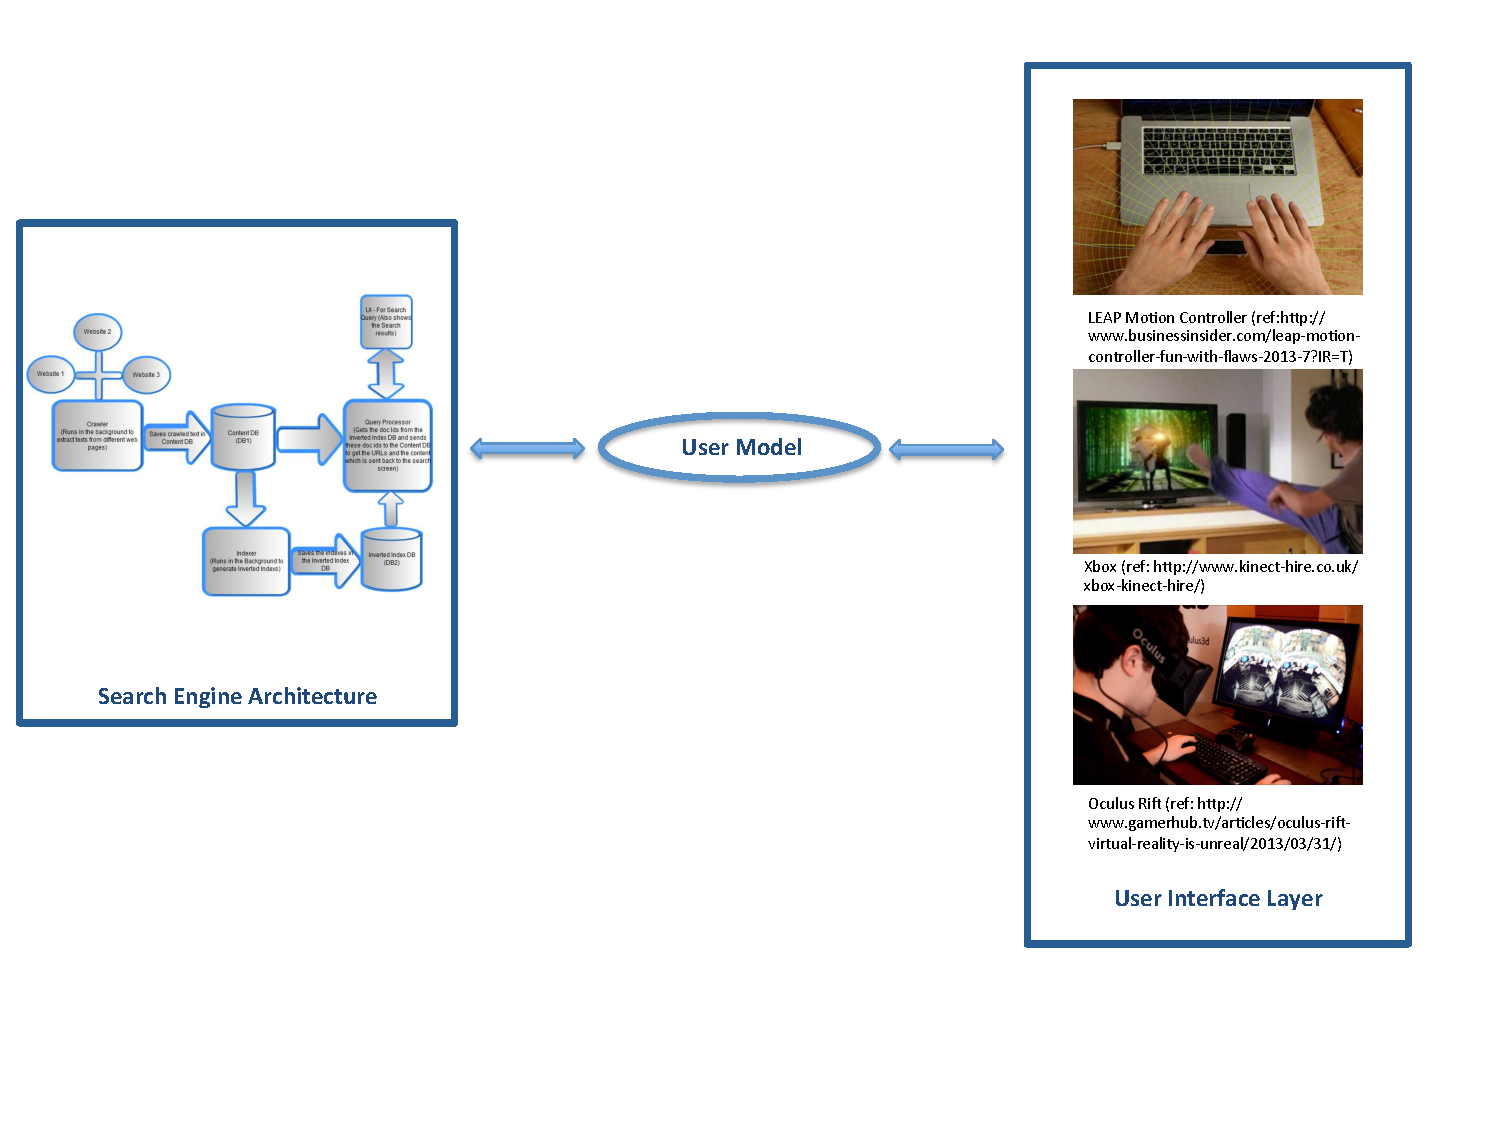
\includegraphics[scale=0.7]{searchEngArchi}
Proposed application: The User Model will be applied to existing Search Engine Architecture\cite{seimage}, and be integrated with a Motion Controlled interface.
\end{center}


\subsubsection{Core Features}
\begin{enumerate}
\item  A web application that synthesises the results from three of the largest and most popular search engines (Google, 67.5\%, Microsoft Bing 18.4\% and Yahoo 10.3\%) \cite{adam}

\item The design and implementation of a stereotyped user model to apply to the search results, and filter them according to specific user needs. The model will return concrete, manageable (not text-overloaded) results, in a consistent manner. The search engine will perform a Key Word In Context search and prioritise results where the key words are used directly, or results have first-order semantic relations to the query words (see Section~\ref{the problem}), i.e., they appear in matched context to the search query.

\item The application will utilise motion controllers to enhance embodiment within search, and enhance the search query process. I will investigate the use of the LEAP motion controller as the main device in the first instance.
\end{enumerate}

\subsubsection{Non-core Features}
\begin{enumerate}

\item Investigating the user preferences for pages with a higher number of pictures. Implement a ranking system for pages with more images to score higher than those with many words. 
\item Investigating the use of the three.Js library for 3D UI (based on WebGL) to integrate with motion controllers.
\item Investigating other motion controller devices (e.g., head-mounted devices).

\end{enumerate}

\subsection{Implementing the Application}\label{api}
\subsubsection{Selecting Existing Search Engines} 
The three most popular search engines (as calculated using an average of the unique monthly visitors) are Google (1,100,000,000 estimated monthly visitors), Bing (350.000.000 estimated monthly visitors) and Yahoo! (300,000,000 estimated monthly visitors)\cite{ebiz}. Google is the most recent and goliath question-answering system (query volume = 64.5\%)\cite{adam}, and the word has become synonymous with the word ‘search’ on the web. This search engine is often considered the most innovative and dynamic, and is the most popular amongst users worldwide (using global traffic rank figures, in March 2015). Yahoo (2003) was the first ever web directory service; it has stronger advertising and e-commerce partnerships and has a query volume of 19.8\%. Bing (Microsoft's answer to search, previously known as msn search), was officially launched in 2005, and has a query volume of 12.8\%, which is substantially less than Google, but nevertheless, is within the top 3 search engines. Other search engines include Ask, AOL, WOW, which will not be included in the search system proposed here in order to limit the redundancy of the search results (of which there will already be a fair amount, see Section~\ref{Existing Combination/Advanced Search Engines}). 

\subsubsection{APIs, Text-Search Libraries}
I will be using the API’s of the three search engines outlined in the above section. Although the same information could be gathered by inspecting the source code for the pages that return the search query results, the API’s were considered to be far more efficient in doing so (e.g., Apache Lucene Key Word In Context is optimised for maximum search efficiency see Section~\ref{apache}). 

\subsubsection{Google Custom Search}
Google Custom Search (GCS) provides a Java API to create a personalised search engine that can be configured to search web pages and images. It works on a pay per search principle. Once signed up, the GCS requires a consumer key and secret, which are hardcoded in the development of the search.\\
The API has methods which (amongst other things) allows the extraction of image search results, page dates, formatting dates, custom snippets, sort by and filter methods. However, this may not be enough, and the GCS API may need to be used in conjunction with a textual-search library in order to reach the goals of this project (the API does not offer Key Word In Context Search in order to trace the contextual information being returned to the user). Costs \$0.01/search.

\subsubsection{Yahoo BOSS}
Just like Google Custom Search, the Yahoo BOSS Java API required the creation of a search engine project (pay per search) with a consumer key and secret. The API is also easy to use and offers the same functionality as the CSC but again is not sufficient alone to reach the goals of the project. Costs \$0.01/search.

\subsubsection{Bing Search API (Data)}
The Bing Search API, similar to Yahoo BOSS and GCS will produce results for Web, Images, News, Videos, Related Search. Bing Search Java API also includes spelling suggestions based on the query entered. Costs \$0.00/search (max 5000 searches/month)

\subsubsection{Faroo API}
Is a free alternative Java API to Google Custom Search API (business), Yahoo BOSS API  (commercial) and Bing Web Search Enterprise (commercial). It offers the possibility to do a Web Search with more that 2 billion pages indexed. Faroo can return news search (articles from newspapers, magazines and blogs) and sort results by publishing date, with author and article image. Trending news pages are also indexed and can be grouped by topic. The API includes suggestions with auto-completes for misspelled items in the search query \cite{faroo}.

\subsubsection{Apache Lucene Library}\label{apache}
Apache Lucene Library is a text-based context search. It is particularly relevant for the current project because it provides powerful, accurate and efficient algorithms to search textual data, the algorithms are scalable and high performance, so will enable users to receive results from their search query with good speed. The API offers the possibility to carry out phrase, wildcard, proximity and range queries which will mean the goals of the project can be fulfilled (Package org.apache.lucene.search.highlight, for the aims of the project refer to ~Section \ref{the problem}). The library also affords ranked searches, with type tolerant suggesters and field searching.

\subsubsection{Key Word In Context} \label{KWIC} 
The Apache Lucene open-source search engine library written in Java allows contextual-text search, also known as Key Word In Context (KWIC)\cite{kwic}. KWIC works by forming an index to allow each word to be searchable. The library takes care of the efficiency of this process, and can return weighted terms of a given query (as an example).


\subsubsection{Google+ API}
Persona (a type of user) development will support the user modeling process by identifying particular characteristics of individuals with Autism in Search. An individual’s personal information pertaining to the persona, will be stored in a Google+ user profile and can be used with the Google+ API (written in Java), containing information such as age, gender, lifestyle, frequent tasks, tools used, and the resources they commonly use. It is also be possible to store information in the 'about me' section on the profile about individual diagnosis (Autism, Asperger, and high/low functioning). This information can be parsed when the query is submitted to the search engine.

\subsubsection{API for LEAP Motion Controller}
Leap Motion SDK offers an API to get tracking data from the Leap Motion Service. A WebSocket interface, allows LEAP Web Based applications, and a WebSocket server listening in on http://127.0.0.1:6437. The user can enable or disable the WebSocket server as they choose to do so, in the device's control panel.
The server sends tracking data in JSON messages and an application can send configuration messages back. This library will be used to establish connection to the server and consume the JSON messages \cite{leap}. 


\subsubsection{ThreeJs Library (Non-Core)}
This javascript library enables WebGL-3D in a web browser. WebGL brings hardware-accelerated 3D graphics to the browser without installing additional software. This library may be used to better integrate the application with the motion controller, and improve the experience of embodiment, and UI of the application.


\subsection{Integrating the Application with Motion Controller Hardware }\label{hardware}
\subsubsection{Hardware Selection Process}
The usability of the hardware will be determined as follows: 
\begin{enumerate}
\item Good timing of the device correlates to a good meaning and a good UX. The LEAP has options to ‘poll’ frames at a constant rate (to keep timing of movement accurate).
\item Cognitive ‘lag’ time. Each of our senses operates with a different lag time. Hearing has the fastest sense-to-cognition/understanding time; sight is the slowest. The device should therefore work with the combinatorial configuration of the senses.
\item As this is a tool to be used with individuals with Autism, the sensory experience of the device cannot be overwhelming.
\item Cognitive-load should not be high (the device is being used to assist with search, so operating the device should not require a great deal of cognitive effort).
\item The device should integrate with concrete behaviours, e.g., drop or grab. 

\end{enumerate}

\subsubsection{LEAP Controller}
The leap controller can recognize and track hands, fingers and finger-like tools. It can report positions, motions and gestures using an infrared light and optical sensors along the x, y and z axes (Cartesian coordinate system). The controller has a 150-degree field of view, and can operate in a range of 1 inch to 2 feet. The API works with distance in millimetre resolution. Time is measured in microseconds, speed in mm/s and angles in radians.

\begin{center}
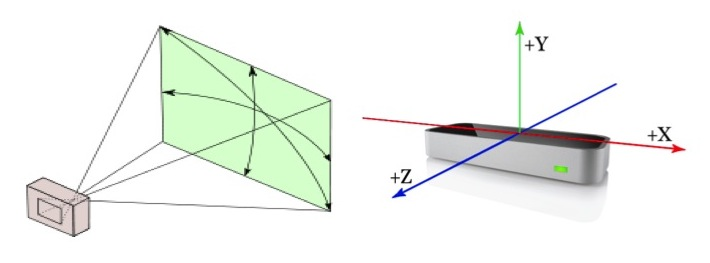
\includegraphics[scale=0.5]{leap}\\
The LEAP controller, with 150 degree view \cite{leap}.
\end{center}

The LEAP uses frames to represent tracked entities such as hands, fingers, tools or gestures. Motion data is recorded as a set of frames (stored, read-only) containing the detected information. 
Frames can be created by calling the Controller.frame(), and up to 60 can be held in the history buffer with the current API. Frames may be 'dropped' if there are resource contrainsts, or, they are missed for example. Once a frame is created, the data can be gathered from the hands(), arms(), fingers(), tools() methods.

\subsubsection{Hands}
The Hand class, returns information about the ID, position of fingers associated with that hand, and arm infomration (left/right).

\begin{center}
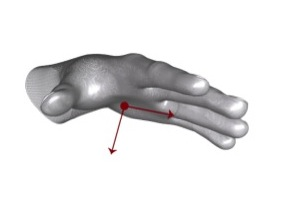
\includegraphics[scale=0.6]{palm}\\
The Hand palmNormal() method and direction vectors define the orientation of the hand \cite{leap}\\.
\end{center}

The software uses parts of visible hand, internal model and previous observations to form a model of the hand. Five finger positions will always be shown but subtle movements of hand, especially if they are tucked up into the hand are harder to detect. For this there is a Hand.confidence() method that provides a rating of how well the observed data fit the internal model \cite{leap}.

\subsubsection{Arms}
The Arms class can return information about orientation, length, width and end points of movements. The LEAP controller software bases these return measurements on previous observations of the user, and using typical human proportions.

\subsubsection{Fingers}
These characteristics are based on the anatomy of the hand, and recent observations. 

\begin{center}
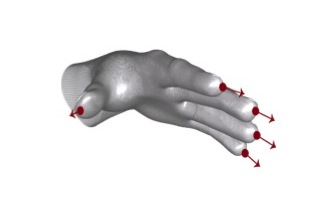
\includegraphics[scale=0.7]{fingers}\\
Finger tip position and direction are given as vectors. \cite{leap}.
\end{center}


\subsubsection{Tools \& Pointables}
Tools can represent any real object (noun), but are longer, straighter and thinner than fingers. Tools must be cylindrical.

\subsubsection{Gestures}
The LEAP recognises certain movement patterns (for each finger or tool individually) allowing the user to indicate an intent. These gestures are observed in a frame and include: CircleGesture, KeyTapGesture, ScreenTapGesture and SwipeGestures.


\subsection{Project Plan}\label{plan}

\subsubsection{Project Timeline}
A high level plan of the project timeline is presented in table ~Table \ref{stages}. The start date of the project is June 5th 2015, and end date is September 13th 2015.
\begin{table}[h]
\caption{Project Stages} 
\centering
\begin{tabular}{ L |c| L}
\hline\hline 
Dates \# & Task & Priority\\ [0.5ex]
\hline 
Jun 05 - Jun 12 & Gather relevant API's \& Libraries & MUST\\
Jun 13 - Jun 19 & Work on synthesis of search results & MUST\\
Jun 20 - Jun 27 & Research \& build user model of Autism & MUST\\
Jun 28 - Jul 06 & Work on configuration with Google+ API& MUST\\
Jul 07 - Jul 14 & Apply user model to Search& MUST\\ 
Jul 14 - Jul 21 & Develop UI & MUST\\
Jul 21 - Jul 28 & Integrate motion controller tools& MUST\\
Jul 29 - Aug 05 & Develop questionnaire and eye-tracker set up & MUST\\ 
Aug 06 - Aug 13 & Test the model and ask for user feedback & MUST\\
Aug 14 - Aug 21 & Revise the user model and UI & MUST\\
Aug 14 - Aug 21 & Develop UI with other motion controllers & COULD\\
Aug 22 - Aug 29 & Develop UI using WebGL/threeJs library & COULD\\
Aug 22 - Aug 29 & Write up project report & MUST\\ 
Early Sep (tbc) & Present findings to supervisor & MUST\\
Sep 13 & Submit report & MUST\\[1ex]
\hline
\end{tabular}
\label{stages} 
\end{table}

\subsubsection{Methodology}
The current project has a relatively short deadline in which a single developer will research and deliver a system prototype and report. The APIs, technology and areas of development are unfamiliar. As the final product depends on user feedback testing, there is an element of uncertainty about what the final product will be/should look like, i.e., a feature could be added/removed at the feedback stage. The characteristics of the current project mean that the most suitable methodology to deliver the application is Agile Methodology. I will focus on development and rapid feedback early in the development, to make changes to the project direction. This methodology works well with the demands and offers the most flexibility and adaptability.


\subsubsection{Development Languages}
I will use Eclipse text editor and attempt to make the application compatible with Google Chrome browser (as it is WebGL-compatible and may be useful for 3D interfaces). The Google, Yahoo, Bing and Apache Lucene APIs are available in Java. The LEAP SDK sends Frame information in JSON format to Web Browsers. As a non-core feature, I may use a 3D interface with the three.Js library which is also JSON format. I will use HTML5 for the development of the Web Application itself. I will use Git for Version Control, JUnit, JSON Test (for testing code) and Mockito (for testing when there are user/external dependencies). \\
JSON is light weight, language-independent data format, and a good tool for sharing data. Importantly JSON offers faster execution and server-side parsing by storing the data in arrays, so that the transfer of data is faster. Faster parsing is particularly important for sharing the LEAP motion controller data. Some of the drawbacks of JSON are that it only has limited support tools available, and little error handling capabilities. It is also vulnerable as it returns responses in wrapped function calls which are vulnerable to attack. Java is a platform and operating-system independent language. It offers a simple, dynamic and robust object oriented, functional language.

\subsubsection{Testing}
\subsubsection{User Testing}
To ascertain whether the goals of the project have been met I will need to test the application with people with Autism. This will include;
\begin{itemize}
\item Recruiting participants to take part in the research. Adolescents and adults with a diagnosis of Autism Spectrum. Recruited from NAS, will be asked to test the application.
\item Obtaining user feedback on the initial product by testing the web search with the LEAP motion controller, with a group of individuals diagnosed with Autism. I will design a questionnaire to test the application's feasibility. If time allows, I hope to use a Tobii Eye-tracker TX300 (in the Department of Psychology, Centre for Brain and Cognitive Development, Birkbeck University of London) to gather high resolution eye-tracking data on the participants as they use the application. This will inform my future developments for revising the application.
\item Revising the model and the ideas to choose the best possible approach/tools to achieve optimization for people with Autism.
\end{itemize}

\subsubsection{Unit Testing}
For testing the application code, I will be using Test Driven Development (TDD). For Java I will use the current version of JUnit (at the time of writing this is 4.12).External dependencies will be mock tested using Mockito. JSON Test will be used to test JavaScript Object Notation \cite{jsontest}. As well as unit testing, Regression testing will be used to testing the project as a whole unit.

\subsubsection{Risks/issues, probabilities and mitigation of impact}
The possible risks associated with the projects development, their impact and how I will attempt to mitigate these risks is outlined in ~Table \ref{risks}. 
\begin{table}[h]
\caption{Risks \& Impact Mitigation} 
\centering
\begin{tabular}{|c | c | L | L |}
\hline\hline 
Liklihood & Impact & Risk & Mitigation\\ [0.5ex]
\hline 
LOW & HIGH & API's require significantly high payment & Find/use alternative\\
\hline 
LOW & HIGH & KWIC library does not offer methods needed to achieve goals of contextual text search & See if I can implement the method, or find additional API\\
\hline 
LOW & MEDIUM & Cannot get research participants with Autism to take part in a usability test & Expand age range of interest in attempt to find participants\\ 
\hline 
MEDIUM & MEDIUM & Google+ API does not configure a user persona/user model well & Use Facebook or alternative\\
\hline 
MEDIUM & HIGH & LEAP does not integrate with web application & Investigate user forums, contact LEAP to source answers, adjust web application accordingly.\\
\hline 
MEDIUM & HIGH & Not enough turn around time to implement the feedback & Develop plan and prototype in time for report submission\\[1ex]
\hline
\end{tabular}
\label{risks} 
\end{table}


\subsection{Summary \& Concluding Statement}\label{future}
I have proposed to research and build a User Model within Search for people with Autism. I presented my research on the downfalls of current search tools, and how they can be improved. I also discussed the use of motion controller hardware (the LEAP) to improve embodiment, UI and UX within Search. I outlined a proposed solution using text and content based libraries to refine search results for this subgroup, based on well-understood aspects of cognition in Autism. I presented my research to date on the tools and resources and methodologies I will draw upon to meet the goals of the project. Last, I outlined the project's timeline.\\
We are moving towards highly personalized information access and retrieval systems. The future of Search will promise the return of user specific results given their needs. Search engines can assist with the forthcoming information-overload problem by exploiting these user models to turn the masses of information available into a specific set of “information goods” for any one user, providing good quality personalized information.

\begin{thebibliography}{100}

\bibitem {gameshealth} Games for Health (2012) Screen-based technologies and Autism. 1: 248-53

\bibitem{moore}Moore, D. J., McGrath, P., \& Thorpe, J. (2000). Computer aided learning for people with autism—a framework for research and development. Innovations in Education and Training International, 37, 218–228.

\bibitem{leap} https://developer.leapmotion.com/ Retrieved 1 April 2015.

\bibitem{briggs}Briggs, Justin. A Better Understanding of Personalized Search. Retrieved 21 April 2014.

\bibitem {Brusilovsky}Brusilovsky, P. and Tasso, C. (2004) User modeling for Web information retrieval. User Modeling and User Adapted Interaction 14 (2-3), 147-157.


\bibitem {CDC}Developmental Disabilities Monitoring Network Surveillance Year 2010 Principal Investigators; Centers for Disease Control and Prevention (CDC). Prevalence of autism spectrum disorders: Autism and Developmental Disabilities Monitoring Network, United States, 2006. MMWR Surveill Summ.2009; 58(10):1–20


\bibitem {Shane and Albert}J Autism Developmental Disorders. 2008 Sep;38(8):1499-508. doi: 10.1007/s10803-007-0527-5. Epub 2008 Feb 22. Electronic screen media for persons with autism spectrum disorders: results of a survey.
Shane HC1, Albert PD.

\bibitem{jsontest}http://www.jsontest.com/

\bibitem{triad}source: http://media.kingdown.wilts.sch.uk/mod/page/view.php?id=7374

\bibitem {Lasater}Lasater, M. W., \& Brady, M. P. (1995). Effects of video self-modeling and feedback on task fluency: A home-based intervention. Education and treatment of children, 18, 389-407.


\bibitem {Pariser}Eli Pariser (2011) First Monday: What's on tap this month on TV and in movies and books: The Filter Bubble by Eli Pariser". USA Today. 2011. Retrieved April 20, 2011. Pariser explains that feeding us only what is familiar and comfortable to us closes us off to new ideas, subjects and important information.

\bibitem{fabienne}Fabienne Samson, Laurent Mottron, Isabelle Soulières, Thomas A. Zeffiro. Enhanced visual functioning in autism: An ALE meta-analysis. Human Brain Mapping, 2011; DOI: 10.1002/hbm.21307

\bibitem{kwic}Manning, C. D., Schütze, H.: Foundations of Statistical Natural Language Processing, p.35. The MIT Press, 1999

\bibitem{seimage}https://insightsdelight.wordpress.com/2012/01/24/inverted-index-the-basic-ingredient-behind-the-recipe-called-search-engine/

\bibitem {Economist} Invisible sieve: Hidden, specially for you. The Economist. 30 June 2011. Retrieved June 27, 2011. Mr Pariser’s book provides a survey of the internet’s evolution towards personalisation, examines how presenting information alters the way in which it is perceived and concludes with prescriptions for bursting the filter bubble that surrounds each user.

\bibitem {MacDuff} MacDuff, Krantz, \& McClannahan (2001). Prompts and prompt-fading strategies for people with autism. In C. Maurice, \& G. Green (Eds.), Making a difference: Behavioral intervention for autism (pp. 37-50). Austin, TX: Pro-Ed.


\bibitem {Sherer}Sherer, M., Pierce, K. L., Paredes, S., Kisacky, K. L., Ingersoll, B., Schriebman, L. (2001). Enhancing conversation skills in children with autism via video technology. Behavior Modification, 25, 140-158.


\bibitem {Thiemann}Thiemann, K. S., \& Goldstein, H. (2001). Social stories, written text cues, and video feedback: Effects on social communication of children with autism. Journal of Applied Behavior Analysis, 34, 425-446.

\bibitem{ebiz}www.eBizMBA.com; 2015

\bibitem {Combining}Combining Search Engines: Existing Solutions Review
http://www.makeuseof.com/tag/4-search-engines-that-combine-google-bing/


\bibitem {Google}Google Remains the most popular search engine http://searchengineland.com/google-worlds-most-popular-search-engine-148089, (2013).  


\bibitem {Vaishnavi1}Sandeep Vaishnavi1 , Jesse Calhou , and Anjan Chatterjee (2001). Binding Personal and Peripersonal Space: Evidence from Tactile Extinction. Journal of Cognitive Neuroscience 13:2, pp. 181–189


\bibitem {adam}Lella, Adam (2014-04-15). comScore Releases March 2014 U.S. Search Engine Rankings. ComScore.com. Retrieved 2015-02-21

\bibitem{bowler}Dermot M. Bowler, Sebastian B. Gaigg, John M. Gardiner (2014) Binding of Multiple Features in Memory by High-Functioning Adults with Autism Spectrum Disorder, Journal of Autism and Developmental Disorders September 2014, Volume 44, Issue 9, pp 2355-2362


\bibitem {googlebing} http://www.makeuseof.com/tag/4-search-engines-that-combine-google-bing/


\bibitem{faroo}http://www.faroo.com/hp/api/api.html\#description

\bibitem{mottron} Laurent Mottron, Jacob A. Burack, Johannes E. A. Stauder, Philippe Robaey (1999) Perceptual Processing among High-functioning Persons with Autism Journal of Child Psychology and Psychiatry 40 (2), 203–211. doi:10.1111/1469-7610.00433

\end{thebibliography}
\end{document}
